\begin{center}
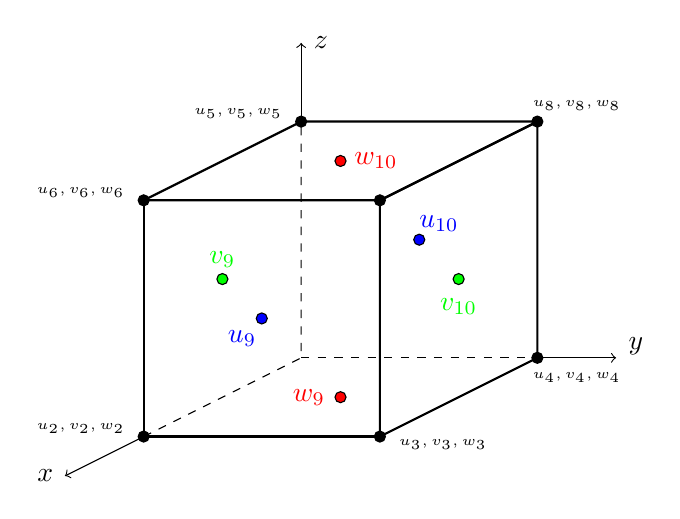
\begin{tikzpicture}
%\draw[fill=gray!23,gray!23](0,0) rectangle (9,7);
%\draw[step=0.5cm,gray,very thin] (0,0) grid (9,7); %background grid

\draw[thick] (2,4.5) -- (5,4.5) -- (7,5.5) -- (4,5.5) -- cycle; %top
\draw[thick] (2,1.5) -- (5,1.5) -- (5,4.5) -- (2,4.5) -- cycle; %front
\draw[thick] (5,1.5) -- (7,2.5) -- (7,5.5) -- (5,4.5) -- cycle; %right

\draw[dashed]   (2,1.5) -- (4,2.5) -- (4,5.5) ; % 
\draw[dashed]   (4,2.5) -- (7,2.5)  ; % 

\draw[thin,->] (2,1.5) -- (1,1); %x
\draw[thin,->] (7,2.5) -- (8,2.5); %y
\draw[thin,->] (4,5.5) -- (4,6.5); %z
\node[] at (0.75,1) {$x$};
\node[] at (8.25,2.65) {$y$};
\node[] at (4.25,6.5) {$z$};

\draw[black,fill=black] (2,1.5)   circle (2pt);
\draw[black,fill=black] (5,1.5)   circle (2pt);
\draw[black,fill=black] (5,4.5)   circle (2pt);
\draw[black,fill=black] (2,4.5)   circle (2pt);
\draw[black,fill=black] (7,2.5)  circle (2pt);
\draw[black,fill=black] (7,5.5)  circle (2pt);
\draw[black,fill=black] (4,5.5) circle (2pt);

\node[] at (1.2,1.6) {\tiny $u_2,v_2,w_2$};
\node[] at (5.8,1.4) {\tiny $u_3,v_3,w_3$};
\node[] at (7.5,2.25) {\tiny $u_4,v_4,w_4$};
\node[] at (3.2,5.6) {\tiny $u_5,v_5,w_5$};
\node[] at (1.2,4.6) {\tiny $u_6,v_6,w_6$};
\node[] at (7.5,5.7) {\tiny $u_8,v_8,w_8$};

\draw[black,fill=blue] (3.5,3) circle (2pt); 
\draw[black,fill=blue] (5.5,4) circle (2pt); 
\node[] at (3.25,2.75) {\color{blue} $u_9$};
\node[] at (5.75,4.2) {\color{blue} $u_{10}$};

\draw[black,fill=green] (3,3.5) circle (2pt); 
\draw[black,fill=green] (6,3.5) circle (2pt); 
\node[] at (3,3.75) {\color{green} $v_9$};
\node[] at (6,3.15) {\color{green} $v_{10}$};

\draw[black,fill=red] (4.5,2) circle (2pt); 
\draw[black,fill=red] (4.5,5) circle (2pt); 
\node[] at (4.1,2) {\color{red} $w_9$};
\node[] at (4.95,5) {\color{red} $w_{10}$};

\end{tikzpicture}\\
\end{center}

